\documentclass[../../main.tex]{subfiles}
% \graphicspath{{\subfix{../images/}}}

\begin{document}
La definición más general acerca del campo de la Inteligencia Artificial (IA) establece que es el área de las Ciencias de la Computación que se enfoca tanto en entender como en crear sistemas que simulen comportamientos \textit{inteligentes}. Si bien existen distintas perspectivas sobre qué significa que una computadora actúe de manera inteligente, la que más ha prevalecido a lo largo de los años es aquel que refiere con la capacidad de computar cómo actuar de la mejor manera posible en una determinada situación \cite{ai-a-modern-approach}. 

En sus comienzos, los métodos desarrollados en el área de la IA estaban principalmente \textbf{basados en conocimiento}, es decir reglas matemáticas formales que permitían a las computadoras llevar a cabo inferencias lógicas y de esta forma resolver problemas que eran intelectualmente difíciles para los humanos \cite{deep-learning}.

Sin embargo, determinar reglas que describan la complejidad y diversidad de la realidad no era una tarea fácil. De esta manera, con el objetivo de hacer a estos sistemas más flexibles y capaces de adaptarse y entender diferentes situaciones, se transicionó hacia un enfoque en el que estos pudieran obtener su propio conocimiento aprendiendo patrones directamente a partir de los datos en lugar de depender exclusivamente de reglas predefinidas. Este cambio de paradigma dio lugar a lo que hoy se conoce como \textbf{Aprendizaje Automático}, la subdisciplina de la IA que permite a los algoritmos mejorar su desempeño en una tarea específica automáticamente a partir de la experiencia. Diversos factores como la creciente disponibilidad de datos, el aumento en la capacidad computacional, y los avances en los algoritmos de optimización \cite{deep-learning} han hecho que esta área sea la que mayor desarrollo e impacto ha tenido durante las últimas décadas. 

Actualmente, la IA abarca una diversidad de tareas, que van desde lo general, como son las habilidades de aprendizaje, razonamiento, y percepción, entre otras; hasta lo específico, como probar teoremas matemáticos, diagnosticar enfermedades, manejar vehículos, mejorar procesos industriales o incluso diagnosticar enfermedades.

\subsection{Aprendizaje Automático (\textit{Machine Learning})}
El Aprendizaje Automático, más conocido por su nombre en inglés \textit{Machine Learning} (ML), es un campo dentro de la IA cuyo objetivo es desarrollar técnicas que permitan que las computadoras \textit{aprendan} automáticamente a partir de la \textit{experiencia}, sin la necesidad de ser explícitamente programadas para hacerlo. Los algoritmos de ML son comúnmente llamados \textbf{modelos}.

En 1997, Tom Mitchell definió en su libro \textit{Machine Learning} \cite{ml-tom-mitchell} el concepto de ``aprender'' de la siguiente manera: ``Se dice que un programa de computadora aprende de la experiencia E con respecto a una clase de tareas T y una medida de desempeño P, si su desempeño en las tareas de T, medido por P, mejora con la experiencia E''. Para tener un mejor entendimiento, nos enfocamos a continuación en cada uno de estos tres componentes.

Las tareas de ML se describen usualmente en términos de cómo el sistema debería procesar un \textit{ejemplo} o \textit{entrada}, entendiendo a esta como un conjunto de características (o en inglés, \textit{features}) medidas cuantitativamente a partir de un cierto objeto o evento \cite{deep-learning}. Dentro de las tareas que pueden ser resueltas por un sistema de ML se encuentran la clasificación, la regresión, la traducción, la detección de objetos en imágenes, la generación de nuevos datos, la detección de valores atípicos, entre muchas otras.

La experiencia hace referencia al tipo de información que el modelo ``puede ver'' durante su proceso de aprendizaje o \textit{entrenamiento} \cite{hands-on-ML-sklearn-tf}. A esta información se la conoce como ``conjunto (de datos) de entrenamiento'', y es un subconjunto de todos los datos con los que se cuentan (\textit{dataset}). En base a la experiencia, los algoritmos de ML se clasifican en dos grandes categorías:
\begin{itemize}
    \item \textbf{Algoritmos de Aprendizaje Supervisado}: experimentan un dataset que contiene pares de entrada-salida, esto es cada ejemplo contiene sus features pero también su ``etiqueta'', que vendría a ser la ``respuesta correcta'' para dicha entrada. El algoritmo aprende una función que asigna (\textit{mapea}) entradas a salidas. Las tareas más comunes llevadas a cabo con este tipo de aprendizaje son las de regresión y clasificación.
    \item \textbf{Algoritmos de Aprendizaje No Supervisado}: ven un dataset que cuenta solamente con características de cada entrada pero sin etiquetas, e intentan aprender automáticamente patrones y propiedades útiles de la estructura de los datos. Algunas tareas que se llevan a cabo con este tipo de aprendizaje son \textit{clustering}, reducción de dimensionalidad, y detección de anomalías.
\end{itemize}
También existen otros tipos de algoritmos, como los de \textbf{Aprendizaje Semi-supervisado}, en donde el dataset contiene algunos ejemplos etiquetados y otros sin etiquetas; y los de \textbf{Aprendizaje por Refuerzo}, en donde el algoritmo aprende la mejor estrategia para una situación a partir de la interacción con su entorno en forma de recompensas y castigos.

Por último, para medir el desempeño de estos modelos, se definen métricas cuantitativas que dependen de la tarea que se esté realizando y del objetivo que se intente lograr. Por ejemplo, en clasificación, una de las más comunes es la de exactitud - \textit{accuracy} -, que es la proporción de ejemplos para los cuales el modelo predijo la salida correcta (dada por el dataset); aunque también existen otras como la precisión, sensibilidad, especificidad, y el puntaje F1. Por otro lado, en tareas de regresión, la métrica que se suele utilizar es la de Error Cuadrático Medio. 

El objetivo fundamental del ML es que un algoritmo actúe correctamente antes nuevas entradas aún no vistas, es decir que \textbf{generalice} más allá de los ejemplos del conjunto de entrenamiento. Por lo tanto, para evaluar qué tan bien se comporta el modelo y poder comparar su desempeño con otros, su rendimiento se mide en otro subconjunto del dataset, distinto con el que aprendió, llamado ``conjunto de test''. Como buen práctica, este conjunto no debe ser mostrado al modelo en ningún momento durante su entrenamiento.

\subsection{Redes Neuronales Artificiales - Aprendizaje Profundo}
Las Redes Neuronales Artificiales (RNAs) son un modelo específico dentro del ML, cuya estructura y funcionamiento están inspirados en los del cerebro. Durante los últimos años, ha sido el área que más desarrollo e impacto ha tenido, principalmente gracias a su versatilidad, potencia y escalabilidad, cualidades que hacen que sean capaces de enfrentar problemas grandes y complejos \cite{hands-on-ML-sklearn-tf}.

% Reseña histórica?
\subsubsection{Breve Contexto Histórico}
Aunque su gran éxito ha sido reciente, lo cierto es que la idea de las RNAs data desde 1943, cuando Warren McCulloch y Walter Pitts presentaron en su artículo ``A Logical Caclulus of Ideas Immanent of Nervous Activity'' un modelo computacional simplificado utilizando lógica proposicional acerca de cómo funcionan las neuronas de cerebros animales en conjunto para llevar a cabo cómputos complejos \cite{hands-on-ML-sklearn-tf}. 

Posteriormente, en 1958, Frank Rosenblatt \cite{rosenblatt1958perceptron} presentó una de las arquitecturas más simples de RNAs: el ``Perceptrón'', el cual sirve principalmente para resolver problemas de clasificación en donde los datos son linealmente separables. Su aporte más notorio es que definió un algoritmo para su entrenamiento.

Más tarde, se descubrió que los problemas que no podían ser resueltos por el Perceptrón, sí podían ser resueltos ``apilando'' múltiples perceptrones, lo cual llevó a la invención del ``Perceptrón Multicapa'' (PMC), también conocido como ``Redes Neuronales de Propagación Directa'' (del inglés \textit{Feedforward Neural Networks}) \cite{deep-learning}. 

\subsubsection{Elementos de una RNA Feedforward}
% Breve Contexto Histórico
% Neurona Artificial
% Función de costo: back-propagation
% Optimizador
% Hiperparámetros: conjunto de validación, cross-validation
% Pesos
% Otras optimizaciones: lotes, detención temprana, dropout


El elemento básico de cualquier red neuronal es la \textbf{neurona}, que es la que lleva a cabo el ``cómputo''. Una neurona está conectada con otras, de las cuales recibe información y a quienes también les envía. Estas conexiones representan las \textbf{sinapsis} y cada una tiene asociada un determinado número llamado \textbf{peso}, que simboliza la intensidad de la conexión. De esta manera, el trabajo que lleva a cabo una neurona es primero computar una suma pesada de sus entradas: \(z = w_1x_1 + w_2x_2 + … + w_nx_n = w^T x\), donde \(x_i\) representa la entrada proveniente de la neurona \(i\) y \(w_i\) es el peso asociado a esta conexión. Y sobre este valor resultante, aplica una \textbf{función de activación} \(h\), siendo como resultado final de la neurona \(h(z) = h(w^T x)\). Esto se puede ver gráficamente en la figura \ref{fig:neuron}.

\begin{figure}[h!]
    \centering
    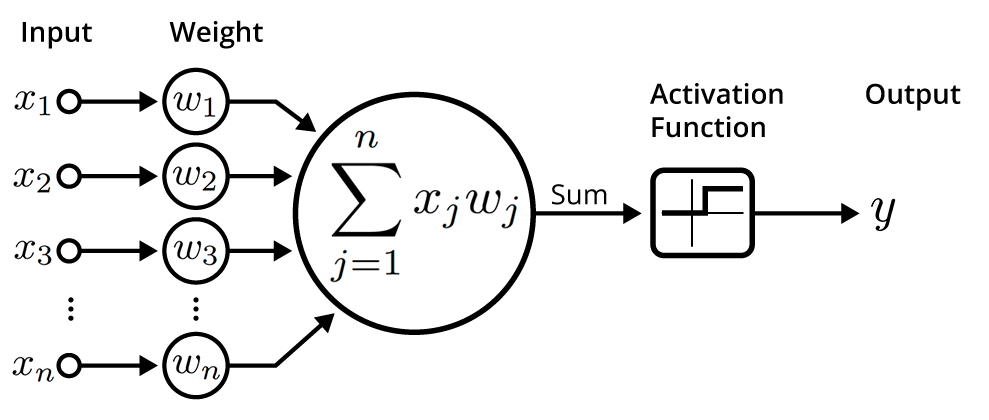
\includegraphics[width=0.35\textwidth]{figs/neuron.png}
    \caption{La neurona computa una suma pesada de sus entradas y aplica una función de activación sobre el resultado.}
    \label{fig:neuron}
\end{figure}

La idea detrás de la función de activación es el hecho de propagar la información proporcionalmente al estímulo provocado por las entradas en la neurona, basándose en la idea de ``disparo'' de una neurona biológica en el momento en que se supera el umbral de activación. La función de activación utilizada en el Perceptrón, uno de los primeros modelos de RNAs, fue la llamada \textit{heavyside}, dada por \(\text{heavyside}(z)=0\text{ si }z < 0; 1\text{ si } z\geq0\). 

Durante los años, se han empleado diferentes funciones de activación, como la sigmoide, la tangente hiperbólica, y la ReLU, dada por \(\text{ReLU}(z)=\text{max}(0, z)\), siendo esta última la más común actualmente.

Dicho esto, una red neuronal está compuesta por diferentes capas de neuronas: la capa de entrada, que es por donde ingresan los datos, una o más capas ocultas o intermedias, en donde aparecen las funciones de activación, y finalmente la capa de salida. En una red \textit{feedforward} particularmente, las neuronas de una capa están conectadas solamente con las neuronas de la capa siguiente, implicando de esta forma que la información fluye solamente en una dirección (de aquí la nomenclatura \textit{feedforward}). Algo a notar también sobre estas redes es que todas las capas están totalmente conectadas entre sí, como puede verse en la figura \ref{fig:neural-net}.

\begin{figure}[h!]
    \centering
    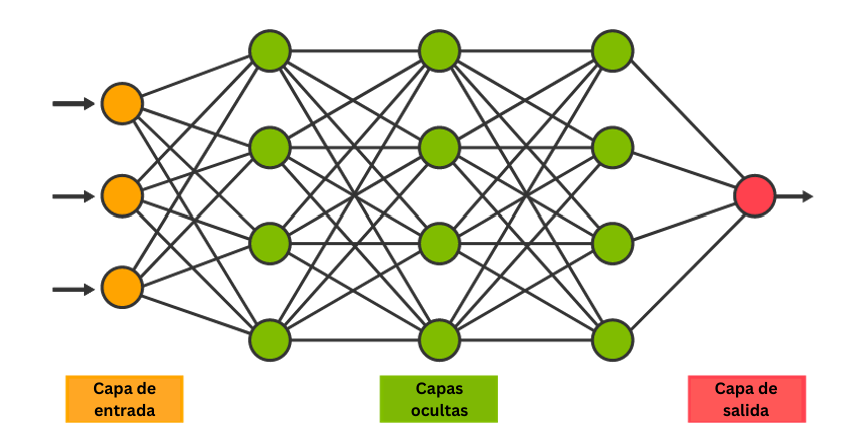
\includegraphics[width=0.6\textwidth]{figs/feedforward.png}
    \caption{Esquema de una Red Neuronal Profunda, con tres capas ocultas. Las neuronas naranjas forman la capa de entrada, las neuronas verdes forman las tres capas ocultas, y las rojas la de salida.}
    \label{fig:neural-net}
\end{figure}

Ahora bien, el objetivo de una red neuronal es \textbf{aproximar una función desconocida} \(g^*\). Para un clasificador por ejemplo, \(y=g^*(x)\) determina una categoría \(y\) para una entrada \(x\). De esta forma, una red define una asignación \(y=g(x; \theta)\) y aprende el valor de los \textbf{parámetros} \(\theta\) que resultan en la mejor aproximación de la función ``oculta'' \cite{deep-learning}. En este caso, los parámetros a aprender por la red serán los pesos sinápticos de todas las conexiones. Matemáticamente, los pesos entre una capa de neuronas y la siguiente se pueden pensar como una matriz \(w\), en donde la entrada \(w_{ij}\) indica el peso sináptico de la conexión entre la neurona \(i\) de la capa ``actual'' y la neurona \(j\) de la capa ``anterior''. La pregunta que surge entonces es \textbf{cómo} hacer para que la red pueda aproximar esta función.

\subsubsection{Entrenamiento de una RNA Feedforward}
A grandes rasgos, el entrenamiento de una red consiste en una suma de \textbf{evaluación} y \textbf{optimización} \cite{pedro-domingos}. Con evaluación, nos referimos al establecimiento de una medida que determine qué tan lejos está el modelo de hallar una buena solución, para lo cual se suele definir una función a minimizar o maximizar llamada \textbf{función objetivo} o \textbf{criterio} \cite{deep-learning}; y la optimización es el método usado para aproximarse a dicha solución, maximizando o minimizando la función objetivo según corresponda.

Cuando lo deseado es minimizar la función objetivo, esta pasa a ser llamada \textbf{función de costo}, \textbf{función de error} o \textbf{función de pérdida}. En problemas de aprendizaje supervisado, esta función compara la salida de la red para determinadas entradas - la predicción - en el estado actual de la red, dado por el valor de los pesos sinápticos en ese momento, con las salidas reales para dichas entradas, dadas por el conjunto de entrenamiento. En resumen, una vez que están fijos los datos del conjunto de entrenamiento, la función de costo es una función de los pesos de la red. Por lo tanto, la denotaremos con \(f(w)\).

Dos de las funciones de costo más utilizadas son el Error Cuadrático Medio y la \textbf{Entropía Cruzada}. De estas dos funciones, nos concentraremos en la última ya que es la más apropiada para problemas de clasificación como el que tratamos. Esto se debe a que mide la diferencia entre la distribución de probabilidad predicha por el modelo y la distribución real de los datos.  En este caso, la capa de salida tiene tantas neuronas como categorías haya, y la salida de cada una de ellas representa el puntaje que le da la red a la categoría correspondiente a cada neurona, donde un mayor puntaje indica una mayor probabilidad de pertenencia de la entrada particular a dicha clase. Para obtener una estimación de la distribución de probabilidad dada por estas salidas, se aplica la función \textit{softmax} \cite{hands-on-ML-sklearn-tf}.

Una vez que se tiene esta función establecida y se calculan las pérdidas para los datos, el algoritmo por defecto que se utiliza para la optimización es el de \textbf{Descenso por el Gradiente} (\textit{Gradient Descent}). Este se basa en modificar los parámetros (i.e. los pesos sinápticos) iterativamente con el objetivo de encontrar mínimos locales de una función, que en este caso será la de costo. Se basa en la idea que la dirección dada por el gradiente es la de mayor crecimiento, y por lo tanto su opuesta es la de menor. De esta forma, lo que se hace en cada paso es calcular el gradiente de la función de costo con respecto a los pesos, y luego actualizarlos siguiendo la siguiente regla:
\[
w = w - \eta \ \nabla f(w),
\]
donde \(w\) representa una matriz de pesos de una determinada capa, y la cantidad \(\eta\) es llamada la \textbf{tasa de aprendizaje}, que determina el tamaño de cada paso. Si \(\eta\) es muy pequeño, entonces el algoritmo tendrá que hacer muchos pasos para converger; pero si es demasiado grande, puede llegar a divergir. 

Actualmente, se utilizan otros optimizadores más sofisticados y eficientes, pero que todos parten de la idea del Descenso por el Gradiente. Los que usaremos en los experimentos son el Descenso por el Gradiente Estocástico (\textit{Stochastic Gradient Descent}, SGD) y Adam (\textit{Adaptive Moment Estimation}), de los cuales se puede leer más en el Capítulo 8 de \cite{deep-learning}.

Ahora bien, recordando que la función \(f\) está fija en todas las entradas y salidas del conjunto de entrenamiento, hay algoritmos de optimización que utilizan todos estos datos para  calcular el gradiente, otros que utilizan de a un ejemplo a la vez para calcular el gradiente y otros que están entre medio de los dos anteriores, es decir utilizan un subconjunto del conjunto de datos para calcular el gradiente (esto es lo que hace SGD). 

Es necesario en este punto introducir el concepto de ``\textbf{época}'' y de ``\textbf{lote}''. Un lote es simplemente una subdivisión de tamaño fijo del conjunto de entrenamiento (o de test). Dicho esto, se llama época al proceso completo en el cual el modelo entrena utilizando \textbf{todos} los datos disponibles en el conjunto de entrenamiento una vez, ya sea recorriéndolos de a lotes o todos de una vez. Si el conjunto está efectivamente dividido en lotes, una época va a consistir de: \textbf{para cada lote}, calcular las predicciones en base a los pesos actuales, obtener los errores de cada muestra del lote, computar los gradientes en base a los ejemplos del lote y actualizar los pesos. Si no, se hacen los mismos pasos pero para todos los datos de una vez.

Al entrenar un modelo, existen ciertos ajustes que son utilizados para controlar su comportamiento llamados \textbf{hiperparámetros}. Los valores de los hiperparámetros no son aprendidos por el modelo \cite{deep-learning}, sino que se fijan de antemano y no se modifican a lo largo del entrenamiento. Algunos de estos son: la cantidad de neuronas en cada capa oculta, la función de activación utilizada en cada capa, el optimizador, la tasa de aprendizaje, el número de épocas, el tamaño de lote, entre otros. Todos estos pueden contribuir a que el modelo mejore su desempeño. Para probar distintos valores de hiperparámetros, que es lo que haremos a continuación, se utiliza un conjunto de datos extra además del de entrenamiento y el de test, llamado de \textbf{validación} que sirve justamente para encontrar los hiperparámetros óptimos.

Otras mejoras que se han implementado para mejorar la eficacia de los modelos, y que emplearemos en los experimentos, son las nombradas a continuación. Por un lado, tenemos la \textbf{detención temprana}, que consiste en frenar el entrenamiento en el último mejor ``estado'' del modelo cuando se observa que a partir de dicho punto el error sobre el conjunto de validación no mejora (notar que cuántas épocas se espera y qué se considera una mejora son nuevos hiperparámetros). Y por otro lado, el \textbf{dropout}, que es un algoritmo que implica suprimir un cierto número de neuronas de una capa de manera aleatoria \cite{apuntes-redes-neuronales}. 

\end{document}